\documentclass{article}
\usepackage{amsmath}
\usepackage{mathtools}
\usepackage{microtype}
\usepackage{tikz}

\usetikzlibrary{decorations.pathmorphing, decorations.pathreplacing, patterns, calligraphy}
\tikzstyle{spring}=[thick,decorate,decoration={zigzag, pre length=0.1cm, post length=0.1cm, segment length=8, amplitude=0.15cm}]

\let\sin\relax
\DeclareMathOperator{\sin}{\smash{\mathrm{sin}}}
\let\arcsin\relax
\DeclareMathOperator{\arcsin}{\smash{\mathrm{arcsin}}}

\setlength\fboxsep{0.2cm}

\author{Derek Garlach}
\title{Harmonic Oscillator}
\date{\today}

\begin{document}
\maketitle
\section{Simple Harmonic Oscillator}
The simple harmonic oscillator comes about, most commonly, from a mass on spring. No friction.
\begin{center}
    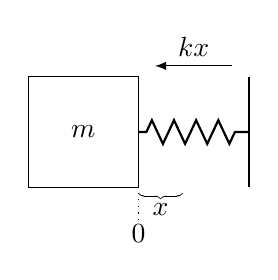
\begin{tikzpicture}[scale=0.7]
        \draw (0,0) rectangle (2,2);
        \node at (1,1) {$m$};
        \draw[spring] (2,1) -- (4,1);
        \draw[thick] (4,0) -- (4,2);
        \draw [decorate,decoration={calligraphic brace,amplitude=0.5ex,mirror,raise=0.5ex}] (2,0) -- (2.8,0) node[midway,yshift=-0.8em]{$x$};
        \draw[latex-] (2.3,2.2) -- (3.7,2.2) node[midway, above]{$kx$};
        \draw[dotted] (2,-0.6) -- (2,0) node[below, yshift=-1em]{0};
    \end{tikzpicture}   
\end{center}
Gives us the differential equation
\begin{equation*}
    m\ddot{x} - kx = 0
\end{equation*}
We solve this equation by solving the characteristic equation
\begin{align*}
    r^2 - \frac{k}{m} &= 0 \\ 
    r &= \pm \sqrt{-\frac{k}{m}}
\end{align*}
Since both $k$ and $m$ are positive
\begin{equation*}
    r = \pm i \sqrt{\frac{k}{m}}
\end{equation*}
and the general solution is
\begin{equation*}
    x = A\cos\!\left(\sqrt{\frac{k}{m}}t\right) + B\sin\!\left(\sqrt{\frac{k}{m}}t\right)
\end{equation*}
We let 
\begin{equation*}
    \omega_0 = \sqrt{\frac{k}{m}}
\end{equation*}
This is both a useful simplification and a meaningful label, the \textit{angular frequency} of the oscillation. we should then rewrite the differential equation
\begin{equation*}
    \ddot{x} - \omega_0^2x = 0
\end{equation*}
And it's solution
\begin{equation*}
    x = A\cos(\omega_0t) + B\sin(\omega_0t)
\end{equation*}
or
\begin{equation*}
    x = A\cos(\omega_0t + \phi)
\end{equation*}
Both of these forms are useful, I will work with both. First one is \textbf{Form 1} and second one is \textbf{Form 2}.
\subsection{Initial Conditions}
We will solve for $A$ and $B$ when given initial conditions
\begin{equation*}
    x(0) = x_0, \qquad \dot{x}(0) = \dot{x}_0
\end{equation*}
\subsubsection{Form 1}
\begin{align*}
    x &= A\cos(\omega_0t) + B\sin(\omega_0t) \\ 
    \dot{x} &= -A\omega_0\sin(\omega_0t) + B\omega_0\cos(\omega_0t) 
\end{align*}
the initial conditions give
\begin{align*}
    x(0) &= A = x_0\\ 
    \dot{x}(0) &=  B\omega_0 = \dot{x}_0
\end{align*}
So the particular solution is
\begin{equation*}
    \boxed{x = x_0\cos(\omega_0t) + \frac{\dot{x}_0}{\omega_0}\sin(\omega_0t)}
\end{equation*}
\subsubsection{Form 2}
\begin{align*}
    x &= A\cos(\omega_0t + \phi) \\ 
    \dot{x} &= -A\omega_0\sin(\omega_0t + \phi) 
\end{align*}
the initial conditions give
\begin{align*}
    x(0) &= A\cos\phi = x_0\\ 
    \dot{x}(0) &= -A\omega_0\sin\phi = \dot{x}_0
\end{align*}
We can get that 
\begin{equation*}
    \cos\phi = \frac{x_0}{A}, \qquad \sin\phi = -\frac{\dot{x}_0}{A\omega_0}
\end{equation*}
So 
\begin{align*}
    \cos^2\phi + \sin^2\phi = 1 &= \frac{x_0^2}{A^2} + \frac{\dot{x}_0^2}{A^2\omega_0^2} \\ 
    1 & = \frac{1}{A^2}\left(x_0^2 + \frac{\dot{x}_0^2}{\omega_0^2}\right) \\
    A^2 & = x_0^2 + \frac{\dot{x}_0^2}{\omega_0^2} \\ 
    A &= \sqrt{x_0^2 + \dot{x}_0^2/\omega_0^2}
\end{align*}
and
\begin{align*}
    \tan\phi = -\frac{\dot{x}_0}{A\omega_0} \frac{A}{x_0} = -\frac{\dot{x}_0}{\omega_0x_0}
\end{align*}
So the particular solution is
\begin{equation*}
    \boxed{x = \cos\!\left(\omega_0t -\frac{\dot{x}_0}{\omega_0x_0}\right)\sqrt{x_0^2 + \frac{\dot{x}_0^2}{\omega_0^2}}}
\end{equation*}
This looks way worse, but it gives the actual amplitude of the wave, and the \textit{actual phase}, whatever thats useful for. So it's physically more useful to look at, as a engineer or something, but it's harder to do math with.

If you let $A^\prime$ and $B^\prime$ be the constants for \textbf{Form 1} of the solution,
\begin{equation*}
    A^\prime = x_0, \qquad B^\prime = \frac{\dot{x}_0}{\omega_0}
\end{equation*}
And then you can relate the two forms as
\begin{equation*}
    A^2 = (A^\prime)^2 + (B^\prime)^2, \qquad \tan\phi = -\frac{B^\prime}{A^\prime}
\end{equation*}
Which is an interesting relation.
\subsubsection{Initial Conditions Sidenote}
Say our initial conditions don't start at $t = 0$, say we have initial condition $x(t_0) = x_0$, we let $t = t^\prime - t_0$ so that
\begin{align*}
    x &= A\cos(\omega_0t + \phi)  \qquad\text{becomes} \\ 
    x &= A\cos\!\big(\omega_0(t^\prime - t_0) + \phi\big) 
\end{align*}
Plugging in the initial condition will still give us the same values for constants $A$ and $\phi$. The fact that the initial conditions don't start at zero just doesn't mean the solution changes, the same things happen, just at a different time. So if need to know what happens a later time, we just shift that time aswell. If we wanted to know that happens at $t = t_1$, then we just plug in $t_1 + t_0$. 
\subsection{Energy}
We find the kinetic energy of our system
\begin{equation*}
    K = \frac{1}{2}m\dot{x}^2 = \frac{1}{2}mA^2\omega_0^2\sin^2(\omega_0t + \phi)
\end{equation*}
recall that $\omega_0^2 = k/m$
\begin{equation*}
    K = \frac{1}{2}kA^2\sin^2(\omega_0t + \phi)
\end{equation*}
and then to potential
\begin{equation*}
    U = \frac{1}{2}kx^2 = \frac{1}{2}k A^2\cos^2(\omega_0t + \phi)
\end{equation*}
And then we can get the total energy
\begin{align*}
    E &= K + U = \frac{1}{2}kA^2\sin^2(\omega_0t + \phi) + \frac{1}{2}k A^2\cos^2(\omega_0t + \phi) \\ 
    E &= \frac{1}{2}kA^2
\end{align*}
The energy is constant, as it should be.
\section{Damped Harmonic Oscillator}
The damped harmonic oscillator comes about when we simple add friction to the mass on a spring. A specific type of friction, \textit{viscous friction}. A type of friction I know nothing about, only that 
\begin{equation*}
    f_\mathrm{visc} = -bv
\end{equation*}
Yeah, cool, whatever. I don't really care. We don't care about viscous friction. We care about a term that is \textit{against} motion, and proportional to velocity. 
Take this and use it.
\begin{center}
    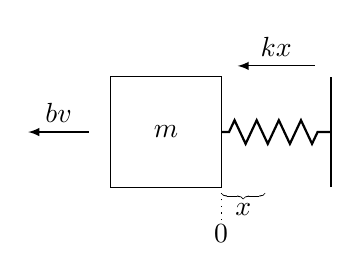
\begin{tikzpicture}[scale=0.7]
        \draw (0,0) rectangle (2,2);
        \node at (1,1) {$m$};
        \draw[spring] (2,1) -- (4,1);
        \draw[thick] (4,0) -- (4,2);
        \draw [decorate,decoration={calligraphic brace,amplitude=0.5ex,mirror,raise=0.5ex}] (2,0) -- (2.8,0) node[midway,yshift=-0.8em]{$x$};
        \draw[latex-] (2.3,2.2) -- (3.7,2.2) node[midway, above]{$kx$};
        \draw[dotted] (2,-0.6) -- (2,0) node[below, yshift=-1em]{0};
        \draw[latex-] (-1.5,1) -- (-0.4,1) node[midway, above]{$bv$};
    \end{tikzpicture}   
\end{center}
Gives us the differential equation
\begin{equation*}
    m\ddot{x} + b\dot{x} + kx = 0
\end{equation*}
Solve it, again, using the characteristic equation
\begin{align*}
    mr^2 + br + k &= 0 \\ 
    r^2 + \frac{b}{m}r + \frac{k}{m} &= 0
\end{align*} 
Yes, the quadratic equation
\begin{equation*}
    r = - \frac{b}{2m} \pm \sqrt{\left(\frac{b}{2m}\right)^{\!2} - \frac{k}{m}}
\end{equation*}
what? this isn't what you expected? \textit{Look Closer}. Anyway, this should be cleaned up, it would be nice if we could keep $\omega_0^2 = k/m$.
\begin{equation*}
    r = - \frac{b}{2m} \pm \sqrt{\left(\frac{b}{2m}\right)^{\!2} - \omega_0^2}
\end{equation*}
If there's anway to simplfy this, it's to pull out an $\omega_0^2$, to get a one, we like ones.
\begin{equation*}
    r = - \frac{b}{2m} \pm \omega_0\sqrt{\left(\frac{b}{2m\omega_0}\right)^{\!2} - 1}
\end{equation*}
Now it's the perfect time to let
\begin{equation*}
    \zeta = \frac{b}{2m\omega_0} = \frac{b}{2\sqrt{km}}
\end{equation*}
\begin{equation*}
    r = - \zeta\omega_0 \pm \omega_0\sqrt{\zeta^2 - 1}
\end{equation*}
An finally it's still worth to let
\begin{equation*}
    \omega_1 = \omega_0\sqrt{\zeta^2 - 1}
\end{equation*}
so
\begin{equation*}
    r = - \zeta\omega_0 \pm \omega_1
\end{equation*}
We apply these substitutions to the differential equation
\begin{equation*}
    \ddot{x} - 2\zeta\omega_0\dot{x} - \omega_0^2x = 0
\end{equation*}
And our solution
\begin{equation*}
    x = Ae^{-(\zeta\omega_0+\omega_1)t} + Be^{-(\zeta\omega_0-\omega_1)t}
\end{equation*}
How nice, except we need to do more work. we know $\zeta$ is always positive, but $\omega_1$ may or may not be complex. If $\zeta > 1$ then $\omega_1$ is real and the solution remains. But if $\zeta < 1$, then $\omega_1$ is complex and we would like to write our solution as
\begin{equation*}
    x = e^{-\zeta\omega_0t}\big(A\cos(\omega_1t) + B\sin(\omega_1t)\big)
\end{equation*}
or
\begin{equation*}
    x = Ae^{-\zeta\omega_0t}\cos(\omega_1t + \phi)
\end{equation*}
If $\zeta = 1$ than $\omega_1 = 0$ and the solution is
\begin{equation*}
    x = (A + Bt)e^{-\omega_0t}
\end{equation*}
Will now analyze all 3 equations
\subsection{Overdamped}





































\end{document}